\subsection*{Redigering af adgangskode} \label{sec:redigrering}
Ud fra app'ens hovedmenu har brugeren mulighed for at tilgå og få vist sine brugeroplysninger samt redigere sin adgangskode. Af \autoref{fig:Redigerbrugeroplysninger} illustreres aktivitetsdiagrammet for redigering af adgangskode.  

\begin{figure}[H]
\centering
\textbf{Aktivitetsdiagram: Redigering af adgangskode}\par\medskip
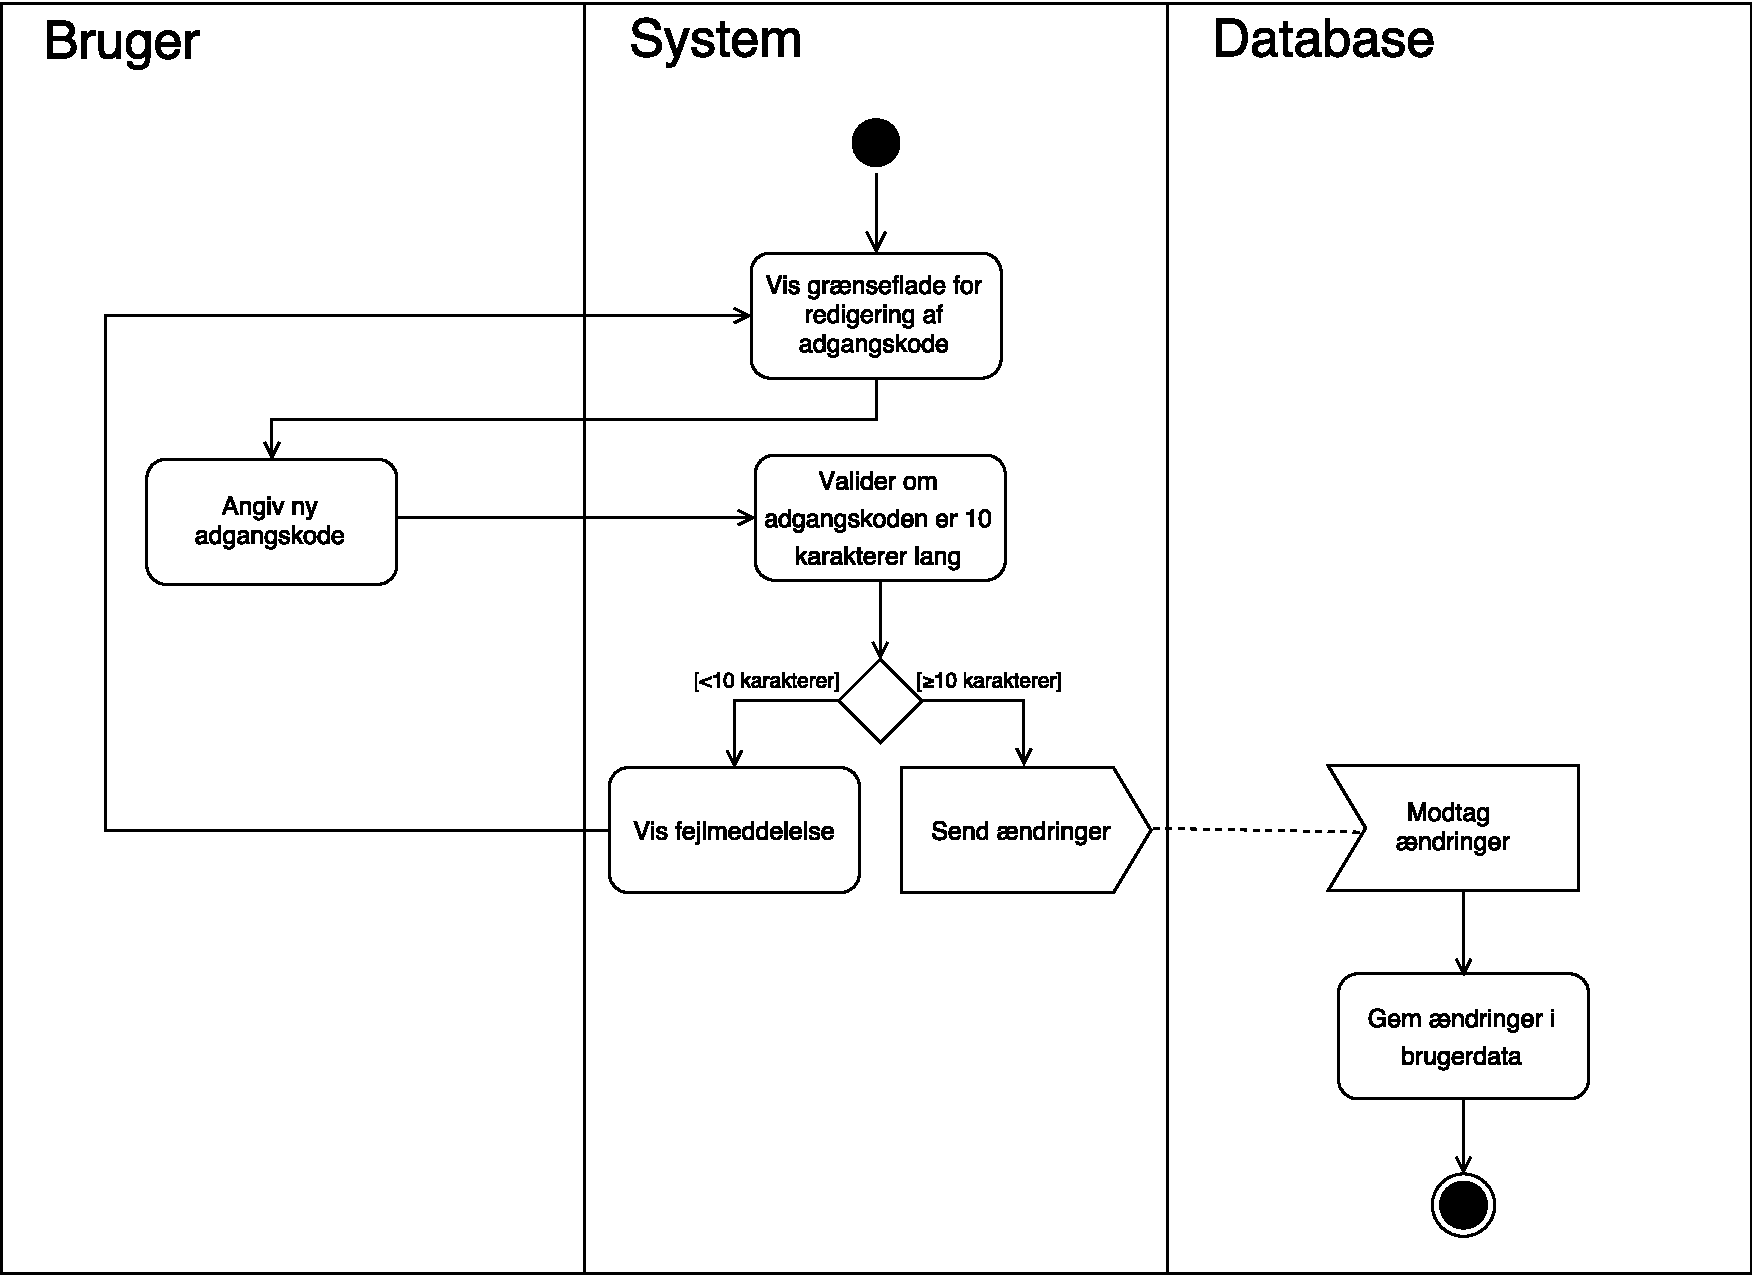
\includegraphics[width=1\textwidth]{figures/aktivitetsdiagram/Redigerbrugeroplysninger}
\caption{Aktivitetsdiagram for redigering af adgangskode.}
\label{fig:Redigerbrugeroplysninger}
\end{figure}

\noindent
Det skal være muligt for brugeren at ændre adgangskode, da brugeren ved oprettelse får tildelt en randomiseret adgangskode. Dertil kan adgangskoden blive personlig for brugeren, hvilket vil gøre det nemmere for brugeren at huske. 
For at den nye adgangskode kan benyttes, skal den minimum være 10 karakterer lang. Rådet for Digital Sikkerhed anbefalder, at adgangskoder bør være minimum 10 karakterer lang, dog er dette ikke et krav \citep{sikkerhed2015}.
Hvis kravet om minimum 10 karakterer ikke opfyldes, sendes en fejlmeddelelse tilbage til brugeren, hvortil en ny adgangskode kan indtastes. 
Ændres adgangskoden sendes ændringen til databasen, hvor den gemmes i databasen.